\section{Corrected Candidate Results}
The domain-separated candidate has 92.876\% accuracy, 95.455\% precision, 90.696\% recall, 93.015\% F1, 98.289\% ROC-AUC and 98.419\% average precision on 31,795 test rows. There are 718 false positives and 1547 false negatives at threshold 0.5. Zero domain overlap is an integrity property, not a promise of near-perfect accuracy.
\begin{figure}[htbp]\centering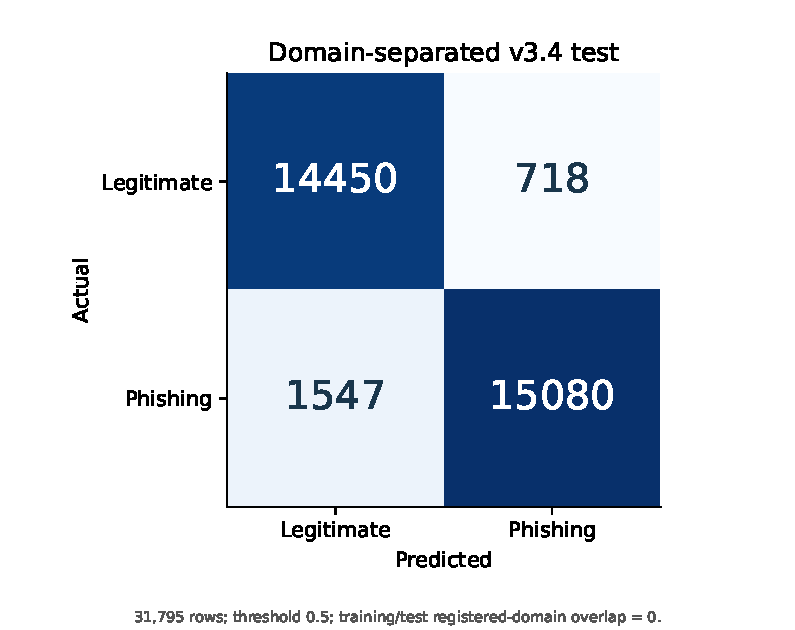
\includegraphics[width=.66\textwidth]{images/confusion_matrix.pdf}\caption{Candidate test confusion matrix}\end{figure}

\section{Common External Snapshot}
The existing fresh2 snapshot has 11,273 rows; two exceed the API's 2,048-character limit. All comparison rates use the remaining 11,271 strings. Before repair, V2 produced 2,177 false positives and 467 false negatives; v3.3 produced 384 and 547. The candidate's external accuracy is 90.578\% and recall 88.232\%. These observations describe different training histories, not a matched architecture ablation.
\begin{figure}[htbp]\centering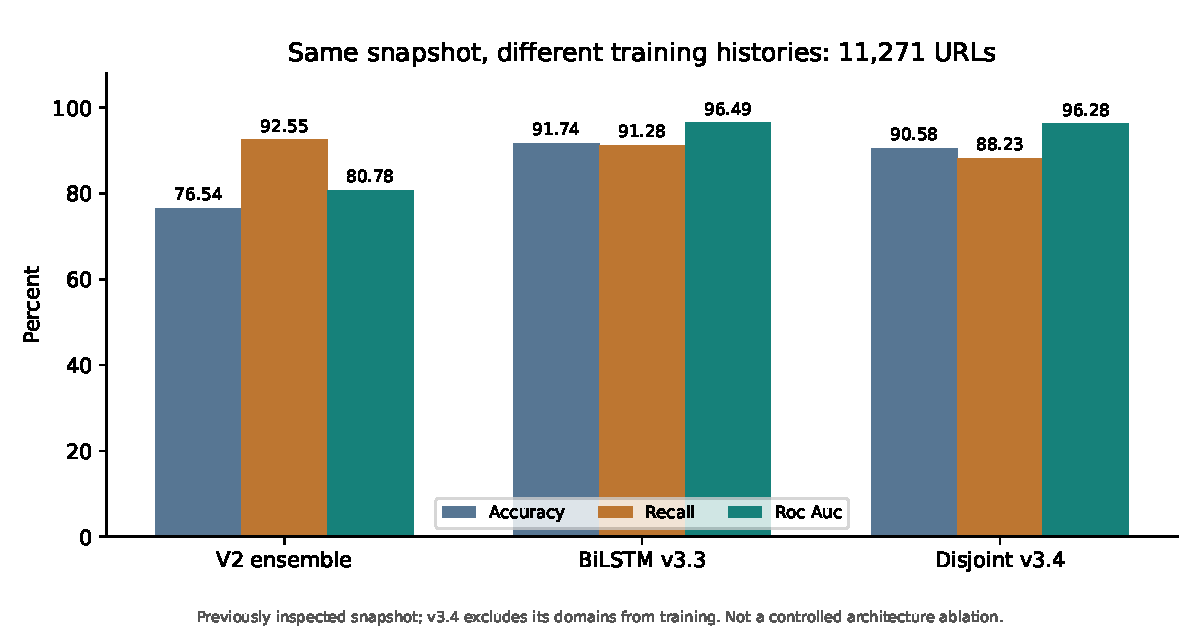
\includegraphics[width=\textwidth]{images/model_comparison.pdf}\caption{Common-input external comparison; snapshot previously inspected}\end{figure}

\section{Adversarial Stress Results}
The old synthetic set contains 1,995 mutated phishing strings and 2,003 unchanged benign strings. V2 misses 9 phishing URLs and v3.3 misses 119. The corrected candidate misses 173, with 91.328\% recall. It was not adversarially fine-tuned during this repair. The historical 37-to-17 result concerns another candidate and cannot be reused as the new model's result.
\begin{figure}[htbp]\centering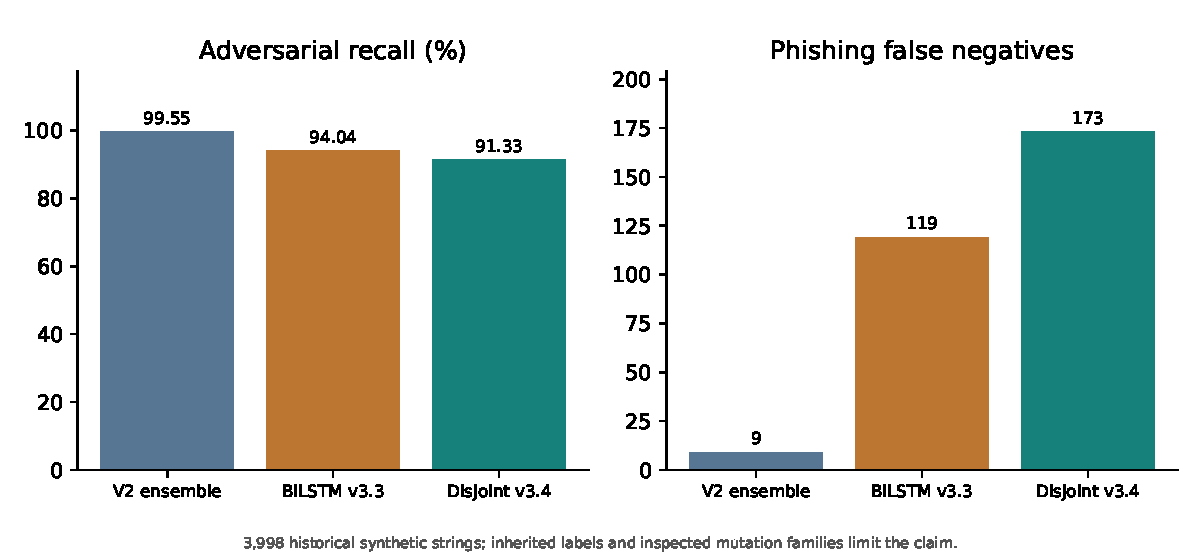
\includegraphics[width=\textwidth]{images/adversarial_robustness.pdf}\caption{Synthetic robustness comparison with explicit false-negative counts}\end{figure}

\section{Training Evidence}
Both losses and validation AUC are saved for the new run. Test scores do not choose an epoch. Figure \ref{fig:history} reflects the recorded history rather than an illustrative curve.
\begin{figure}[htbp]\centering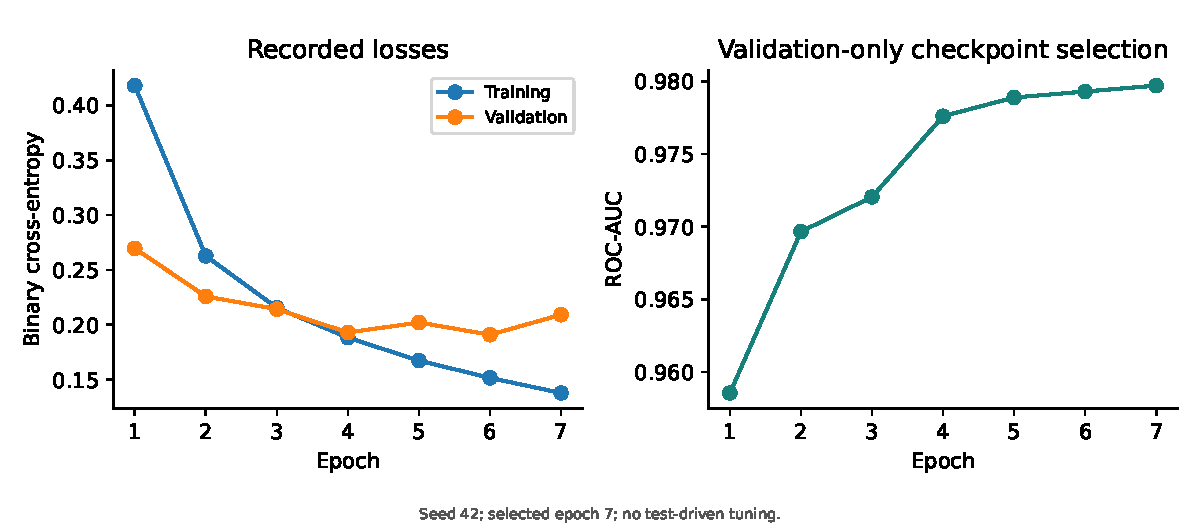
\includegraphics[width=\textwidth]{images/training_history.pdf}\caption{Actual v3.4 training history}\label{fig:history}\end{figure}

\section{Reference Study and Historical Reproduction}
The paper reports 99.819\% accuracy, 100\% precision, 99.635\% recall and 99.947\% ROC-AUC. Our first 20,000-URL reproduction reports 99.525\%, 100\%, 99.048\% and 99.931\% respectively on its 3,998-row test. The candidate values above use a different corpus and partition. These numbers are separately labelled and are not used to claim that one study dominates another. Complete current comparisons, including PR-AUC, FP and FN, are stored in \texttt{docs/evidence/latest\_model\_comparison.csv}.